%%%%%%%%%%%%%%%%%%%%%%%%%%%%%%%%%%%%%%%%%%%%%%%%%%%%%%%%%%%%%%%%%%%%%%%%
%                                                                      %
%     File: Thesis_Background.tex                                      %
%     Tex Master: Thesis.tex                                           %
%                                                                      %
%     Author: Andre C. Marta                                           %
%     Last modified :  2 Jul 2015                                      %
%                                                                      %
%%%%%%%%%%%%%%%%%%%%%%%%%%%%%%%%%%%%%%%%%%%%%%%%%%%%%%%%%%%%%%%%%%%%%%%%


\chapter{Background}
\label{chapter:background}
In this chapter, we start by introducing the vulnerabilities considered in this thesis. Then, we present taint analysis and describe a few static and dynamic approaches that somehow try to solve the problem of portability.


%%%%%%%%%%%%%%%%%%%%%%%%%%%%%%%%%%%%%%%%%%%%%%%%%%%%%%%%%%%%%%%%%%%%%%%%
\section{Input Validation Vulnerabilities}
\label{vulnerabilities}
This section briefly presents a list of vulnerabilities considered in this work. We can divide them in four categories \cite{iberia} - \textit{query manipulation, client-side injection, file and path injection} and \textit{command injection}. The main problem of all these vulnerabilities lies in the improper validation of user input. Our work focuses on this kind of vulnerability.

\subsection{Query Manipulation}
These vulnerabilities are associated with the construction of queries or filters that are executed by some other engine (e.g., a database management system). If the query is constructed with unsanitized inputs, then it is possible to modify the normal behavior. 

All vulnerabilities in this category can be prevented by sanitizing user input, so it does not contain meta-characters that can alter the behavior of the engine.


\subsubsection{SQL Injection} 
This vulnerability is caused by the use of string building functions to create SQL queries. An attack consists of mixing normal characters with meta-characters. In the example of listing \ref{phpsql}, a malicious user can provide a username \texttt{"admin' ---"} causing the query to execute without the need of a password.  

\begin{lstlisting}[language=PHP,
    showstringspaces=false,
    caption={PHP code vulnerable to SQL Injection},
    label=phpsql, float]
$name = $_GET['username'];
$pass = $_GET['password'];
$query = "SELECT * FROM users WHERE name='$name' AND password='$pass'"; 
$result = mysql_query($query);
\end{lstlisting}


\subsubsection{NoSQL Injection} Non-relational (NoSQL) databases are used in many large-scale web applications. There are several NoSQL database engines that implement them. MongoDB \cite{Mongo:online} is the most popular engine implementing the document store model \cite{DBEngine7:online}, so we will focus on vulnerabilities from web applications that connect to a MongoDB instance. Mongo executes queries in JSON format, so a NoSQL Injection (NoSQLI) vulnerability is caused by the use of string building functions to create the JSON query.


\begin{lstlisting}[
    showstringspaces=false,
    caption={JavaScript code vulnerable to NoSQL Injection},
    label=jsnosql]
let username = req.query.username;
query = { $where: `this.username == '${username}'` }
User.find(query, function (err, users) {
    res.render('userlookup', { title: 'User Lookup', users: users });
});
\end{lstlisting}


Listing \ref{jsnosql} shows an example of code vulnerable to NoSQLI. 
In the example, the program takes the username query parameter from the request URI and inserts it in the query. The program then sends the query to the database and returns to the user the result of the query. In this example, if a user passes as argument a string like \texttt{' || 'a'=='a} the query will become \texttt{\$where: `this.username == '' || 'a'=='a'`} which will naturally evaluate to true, and thus returning all values. To remove this vulnerability it is enough to sanitize or escape the user input.


\subsubsection{XPath Injection} This vulnerability is very similar to SQL Injection, but in this case, the data is injected in XML documents, which are often used to store data or configurations. Listing \ref{xpath} shows an example of a PHP script vulnerable to XPath injection. The script takes a username and a password (lines 2, 3) and inserts them into an XPath query (line 4).
An attacker could provide as username \texttt{admin' or 1=1}, causing the script to return information about the admin user without providing a password.
To prevent this vulnerability, it is enough to check if the input contains malicious characters.


\begin{lstlisting}[language=PHP,
    showstringspaces=false,
    caption={PHP code vulnerable to XPath Injection},
    label=xpath, float]
$users = simplexml_load_file("users.xml");
$name = $_POST[’username’];
$pass = $_POST[’password’];
$query = "//User[UserName/text()='".$name."' And Password/text()='".$pass."']";
$result = $users->xpath($query);
\end{lstlisting}

\subsubsection{LDAP Injection} 
LDAP (Lightweight Directory Access Protocol) injection is also exploited by providing meta-characters to string-building functions. LDAP Injection attacks aim to modify the structure of the filter and retrieve data from a directory.

\subsection{Client-Side Injection}
The vulnerabilities in this category allow an attacker to execute malicious code in the victim's browser. This kind of attack is not against the application itself but against the user and can be prevented by either sanitizing or encoding the input.
\subsubsection{Cross-site scripting (XSS)}
There are three types of XSS attacks: reflected or non-persistent, stored or persistent and DOM-based.
A program vulnerable to reflected XSS can have a single line, \textit{"echo \$\_GET['user'];"} 
The attack consists of convincing the user to click on a link to the web application with a malicious script which will be reflected by the \textit{echo} instruction. (e.g., \textit{www.a.pt?user=<script>*malicious code*</script>}).
A stored XSS consists of two steps: first, the attacker inserts a malicious script in the server, then later, the server returns that script to one or more users.

\subsubsection{Header injection} This vulnerability allows an attacker to break the HTTP  response with \textit{"\textbackslash n"} and \textit{"\textbackslash r"}. This allows the attacker to inject malicious code in headers or even a new HTTP  response. It can be avoided by sanitizing these characters.

\subsubsection{Email injection} Very similar to Header Injection, it has the goal to manipulate email components (e.g., sender, destination, message) by injecting the line termination character. In this case, sanitizing the input solves the problem as well.

\subsection{File and Path Injection} This category considers vulnerabilities related to file accesses from web applications, the file system and to URL locations different than the web application.

\subsubsection{Remote file inclusion} PHP allows a script to include files, which can be vulnerable if the file name comes from user input. In the example of listing \ref{rfi}, if a malicious user provides as parameter \textit{country} the URL \textit{http://www.site.pt/hack}, would cause the execution of \textit{hack.php} in the server.  


\begin{lstlisting}[language=PHP,showstringspaces=false, caption={PHP script vulnerable to remote file inclusion},label=rfi,captionpos=b]
$country = $_GET['country'];
include($country . '.php');
\end{lstlisting}

Encoding the input or making it impossible for a user to deliberately influence the filename prevents this vulnerability.

\subsubsection{Directory/Path traversal} This vulnerability allows an attacker to read arbitrary files from the server. To access them the attacker builds an URL containing path metacharacters, such as ".." and "/". In the example of listing \ref{rfi}, if \textit{"../../../etc/passwd\%00"} is passed as input, the file \textit{"/etc/passwd"} is sent to the attacker  (the null character \%00 truncates additional characters, .php in this case).

\subsection{Command injection} 
This category consists of vulnerabilities that allow an attacker to inject operating system commands or PHP code directly. 

\subsubsection{OS command injection}
This vulnerability consists of executing arbitrary system commands defined by the attacker. Consider the following example that uses a script to count the words of a file: \textit{"\$words = shell\_exec ("/usr/bin/wc" . \$GET\_['file']);"} (\textit{shell\_exec} executes system commands and \textit{wc} is a system command to count words). An attacker could retrieve a file from the server by giving as input \textit{"file.txt; cat /etc/passwd"}. The resultant instruction \textit{"\$words = shell\_exec("/usr/bin/wc file.txt; cat /etc/passwd);"} executes the \textit{wc} and \textit{cat} commands. The second command shows the content of a file.

\subsubsection{PHP code injection}
This vulnerability is caused by the \textit{eval} function in PHP. This function runs the code that it receives as a string in its parameter. Consider the example from listing \ref{phpcodeinjection} that uses the \textit{eval} function to concatenate the string \textit{"Hello"} with the name provided by the user. The attacker can do a command injection attack by providing a username and a command separated by a semicolon (e.g., \textit{"Bob; cat /etc/passwd"}). To avoid this attack, the input must be sanitized, but it is not that simple. For this reason, the use of \textit{eval} function is not advised.


\begin{lstlisting}[language=PHP,showstringspaces=false, 
  caption={PHP script vulnerable to code injection},label=phpcodeinjection,captionpos=b]
$msg = 'Hello';
$x = $_GET['username'];
eval('$msg =' . $msg . $x . ';');
echo $msg;
\end{lstlisting}


%%%%%%%%%%%%%%%%%%%%%%%%%%%%%%%%%%%%%%%%%%%%%%%%%%%%%%%%%%%%%%%%%%%%%%%%%%%%%%%%%%%%%%%%%


\section{Vulnerability detection}
\label{relatedwork}
There are many different approaches to prevent injection vulnerabilities. A very popular one is \textit{taint analysis} which can be divided in two categories: \textit{static taint analysis} and \textit{dynamic taint analysis} \cite{schwartz2010all}. In this thesis, we will focus on the first one to detect vulnerabilities. There is also a second type of dynamic prevention which is \textit{parse tree validation} \cite{sqlparsetree1,sqlparsetree2}.

\subsection{Taint analysis}
\label{taintanalysis}

This technique consists of tracking the flow of sensitive information by marking user input as \textit{tainted} and then propagate the \textit{taint marks} recursively to the variables that are influenced by other \textit{tainted} data. Then, it checks if \textit{tainted} data reaches \textit{sensitive sinks}. If it does, there is a vulnerability that could be exploited.

\textit{Taint analysis} has three main components:
\begin{enumerate}
    \item \textit{Data entry point} - the input that comes from untrusted sources is marked as \textit{tainted};
    \item \textit{Taint propagation} - the \textit{taint} marks are then propagated according to a propagation policy;
    \item \textit{Sensitive sinks} - Every function that can be exploited (e.g., \textit{eval()},  \textit{my\_sql\_query()}). The tools then check if the data that enter \textit{sensitive sinks} is \textit{tainted}  or not.
\end{enumerate}

There are two types of taint propagation policies: \textit{explicit} and \textit{implicit information flow}.
Listing \ref{explicit} is an example of \textit{explicit information flow}. Assume that the value of the parameter \textit{a} is tainted, then the taint will be propagated to variable \textit{w} since \textit{a} is involved directly in the computation of \textit{w};

The second type of taint propagation is less intuitive. It refers to situations in which a tainted value affects the value of another variable indirectly. Consider the code in listing \ref{implicit} and assume the value of parameter \textit{a} is tainted. Although \textit{a} is not involved directly in the computation of the value of variable \textit{x}, the value of \textit{a} affects the value of \textit{x} through dependency control.


\begin{lstlisting}[language=C, caption={Explicit information flow},label=explicit,captionpos=b]
void foo(int a){  
    int w;
    w = a * 2;
}  
\end{lstlisting}

\begin{lstlisting}[language=C,caption={Implicit information flow},label=implicit,captionpos=b]
void foo(int a){
    int x;
    if (a > 5){
        x = 1;
    }
    else{
        x = 2;
    }
    print(x);
}
\end{lstlisting}


\section{Static Analysis Tools}
\label{static}
Static analysis tools use pointer and taint analysis to find data flows from \textit{entry points} to \textit{sensitive sinks}. They can also verify if a \textit{sanitization function} is called on tainted inputs. Since \textit{static taint analysis} must make a lot of simplifications, it is prone to false positives and negatives. 
However, since it can be applied to either source or compiled code, static analysis tools are often used to automate the detection of bugs and vulnerabilities. Nowadays, they are often part of the development process, with their use being automated by continuous integration pipelines \cite{mohammad2016continuous}. The reason is that they are a cheap way of detecting issues in code, giving the developers more confidence in their software. Next, we discuss some static analysis tools.

%%%%%%%%%%%%%%%%%%%%%%%%%%%%%%%%%%%%%%%%%%%%%%%%%%%%%%%%%%%%%%%
\subsection{Micro-grammars analysis}

F. Brown, A. Notzli, and D. Engler \cite{microgrammars} managed to implement an effective bug-finding static checker, which is a static analysis tool that has the goal to find bugs in a program (e.g., \textit{null pointers}, \textit{deadlocks}), and that it is orders of magnitude less complex than traditional checkers. 
They achieved this improvement by using a new source code parsing technique based on incomplete \textit{micro-grammars}, instead of depending on every syntax detail of a language or its compiler.

Traditional checking systems use parsers designed to parse a complete language syntax, thus rejecting any input that does not lead to a valid parse. On the other hand, micro-grammars parsing for bug finding has two main differences from traditional parsing.

\begin{enumerate}
  \item When a traditional parser finds a non-matching input to its specifications, it returns an error. By contrast, when a micro-grammar parser hits a non-matching input, it simply slides forward by one token and tries again. This approach is called \textit{sliding window}, and it allows the parser to match all the specifications described by the micro-grammar without getting stuck and skip all those that do not match, consuming all the input. 
This way their static checker only focuses on the most important aspects of a language, which it is used to detect bugs, and ignores the rest. 


\item  Micro-grammars allow developers to perform fine-grained input skipping by using \textit{wildcard} non-terminals that lazily match any input up to a suffix. For example, the micro-grammar ``\textit{S  \( \rightarrow \) if (wildcard)}" when applied to a file with five \textit{if} statements produces five parse trees where lists of tokens match to each \textit{wildcard} node. For example, parsing ``\textit{if (x == 1)}" would result in a normal \textit{if} node and a \textit{wildcard} node containing ``\textit{["x", "==", "1"]}". On the other side, a traditional parser creates a tree with one node for every token.
\end{enumerate}


Wildcards are implemented based on the \textit{SkipTo(P)} rule, represented in Figure \ref{skipTo}, which skips tokens until it reaches a suffix \textit{P}. Figure \ref{skipTo} also shows a micro-grammar example where \textit{Rule1} accepts any token that starts with the character \textit{a} and ends with \textit{cd}. It would accept \textit{abcd} for example, but not \textit{abd}. 

The \textit{Slide'} rule, which corresponds to \textit{Sliding Window} implementation, slides one token until it can find something to accept. Because of this rule, \textit{Rule1} is able to accept inputs such as \textit{"Xabcd"}, even though the input does not start with the character \textit{a}.
 
\begin{figure}
\centering
\begin{minipage}{.5\linewidth}
\textit{AnyToken} \( \rightarrow \) \textit{token, token \(\in\) language}\\
\textit{SkipTo(P)}  \( \rightarrow \) \textit{P | AnyToken SkipTo(P)} \\
\textit{Slide'} \( \rightarrow \) \textit{SkipTo(P) Slide' |  \(\epsilon\)} \\
\textit{Rule1} \( \rightarrow \) \textit{a SkipTo(cd)}
\end{minipage}    

\caption{\textit{Wildcard} and \textit{Sliding Window} micro-grammar}
    \label{skipTo}
\end{figure} 


The implementation of this static checker is very modular and it is composed of a lexer,  parsers and checkers. The parsers are recursive and also modular. There is a parser for each non-terminal, for example the parser for \textit{C} is composed by smaller parsers for \textit{if} statements, \textit{while} loops, \textit{for} loops, etc. Then all these small parsers compose the parser for \textit{C}. This modularity brings another big advantage, the possibility of reusing a lot of these small parsers between languages, for example, \textit{C} and \textit{Dart} share many parsers.

According to the authors, to extend their static checker to another language, one has to do the following: \begin{enumerate}
    \item Specify a lexer by supplying a list of keywords, operators, and a set of regular expressions for identifiers, literals and comments. A typical specification is around ten lines of code.

    \item Build parsers recursively for each non-terminal. In this step, the developer may be able to reuse parsers from another language with similar syntax.
    
    \item Develop checkers.
\end{enumerate} 

The use of micro-grammars and the architecture modularity makes the tool relatively easy to port to other languages.

The static checker presented in the paper focuses on a specific style of bug checking, called \textit{belif-style}. This style assumes that programmers do not want to crash their programs, so from this, we can extract beliefs which are facts implied by the code. For example, the operation \textit{x/y} implies that \textit{y} can not be 0. Therefore, if there is a flow that contradicts this belief, it is considered that there is an error.

The fact that this approach does not depend on every detail of the language somehow inspired our work.
%%%%%%%%%%%%%%%%%%%%%%%%%%%%%%%%%%%%%%%%%%%%%%%%%%%%%%%%%%%%%

\subsection{SonarQube}
SonarQube \cite{campbell2013sonarqube} is a widely used commercial static analysis tool. Performs static analysis based on a set of rules that can be defined by the user. It is able to detect bugs (e.g., possible \textit{null references}) or bad practices in source code (e.g., empty \textit{catch} blocks in Java). Furthermore, it also performs static taint analysis to find vulnerabilities. The taint analysis supports 4 languages, while other features support more than 20. However, since SonarQube is a commercial tool and it is not open source, we can not make any assertion about its complexity. 


\subsection{FlowDroid} FlowDroid \cite{arzt2014flowdroid} is a precise static taint analyzer specifically tailored for Android and Java applications. Analyzes apps' bytecode and configuration files to find vulnerabilities. FlowDroid is precise because it models the lifecycle of android apps and it is context, field, object and flow-sensitive. 


\subsection{Pixy}
Pixy \cite{jovanovic2006pixy} is one of the first tools that processes PHP code. It performs taint analysis on PHP source code and extends it by using \textit{alias analysis}, which takes into account the existence of aliases i.e., of two or more variable names that reference the same variable. It is able to detect SQL injection and Cross-site scripting in PHP code that does not use objects.

\subsection{Andromeda}
Andromeda \cite{tripp2013andromeda} is a demand-driven static taint analysis tool that supports Java, C\# and JavaScript. It is flow and context-sensitive. Furthermore, it extends its analysis by being integrated with Framework For Frameworks (F4F), which is a solution for augmenting taint analysis with precise framework support \cite{sridharan2011f4f}. 


\section{Dynamic Analysis Tools} 
\label{dynamic}
Dynamic taint analysis tools instrument applications with the ability to track the source of inputs in runtime. The applications are then able to determine if the data that reaches \textit{sensitive sinks} contain any untrusted (\textit{tainted}) inputs. Furthermore, \textit{dynamic analysis} can also check whether input sanitization was done correctly or not, contrary to \textit{static analysis}. Since \textit{dynamic taint analysis} is done at runtime, analyzing applications results in adding performance overhead.


\subsection{Dytan} 

Dytan \cite{dytan} is a dynamic taint analysis framework that aims to be generic and customizable. It is a very precise tool since it does taint tracking at a byte level, meaning that it can tell exactly which byte of a variable is tainted. It instruments compiled code (\textit{x86}) with \textit{taint tracking} ability, so it does not depend on the availability of the source code. Furthermore, it supports both \textit{explicit} and \textit{implicit information flow} propagation. In the article, the authors successfully use Dytan to detect SQL Injection, buffer overflows and format string attacks.

Dytan allows users to specify three main aspects of the analysis:
\begin{enumerate}
    \item \textit{Taint Sources} - Allows to set which sources are to be marked as \textit{tainted}. The user can choose from variables, memory offsets, data from specific functions, from a type or specific I/O streams.
    \item \textit{Propagation Policy} - User can choose between two different propagation policies: 
    \begin{itemize}
        \item \textit{Explicit information flow} - a tainted variable is directly involved in the computation of another variable's value.
        \item \textit {Implicit information flow} - a tainted variable affects the value of another indirectly, through information flow.
    \end{itemize}
    \item \textit{Taint Sinks} - The user can set variables, functions, function parameters or instructions (ex \textit{jump};) as \textit{sensitive sinks}.
\end{enumerate}

In spite of being customizable, it is still bound to compiled code, so it can not be applied to an interpreted language or to languages that compile their code to an intermediate language, such as Java or C\#. Furthermore, since the granularity of its taint tracking is a byte, it adds a runtime slowdown ranging from 30x-50x (where a slowdown of 1x means that the system now takes twice as much time to run). This makes the tool inviable to be run in real-world systems. 

Another reason for this huge overhead is that Dytan taint tracks all implicit flows, which generates a lot of unnecessary taints. Dta++ \cite{dt++} presents an improvement to this problem by identifying a minimum set of implicit flows in the program that potentially cause under-tainting, and then generate \textit{taint} propagation rules to solve it.


\textit{Taint Check} \cite{taintcheck} is a tool similar to Dytan. It also instruments compiled \textit{x86} code, but it is inferior compared to Dytan because it only detects buffer overflows and string format attacks and also lacks customizability.



\subsection{Phosphor} 
Phosphor \cite{phosphor} is a more recent tool, that implements \textit{taint tracking} for two JVM (Java Virtual Machine) based languages: Java  and Scala. It does it by instrumenting \textit{bytecode}, without requiring the source code. This way \textit{Phosphor} is able to run on top of unmodified JVMs (Figure \ref{phosphorfig} shows its high-level architecture).

\begin{figure}[h]
\centering
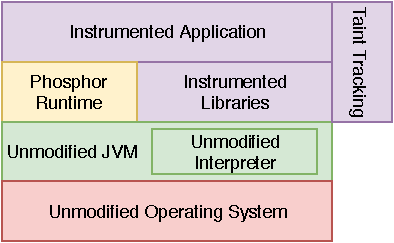
\includegraphics[scale=1]{images/PhosphorArchitecture.pdf}
\caption{\textit{Phosphor's} high-level architecture} \label{phosphorfig}
\end{figure}

It has two main differences from Dytan: 
\begin{itemize}
    \item It does tracking at variable level instead of byte level.
    \item It does not support \textit{implicit information flow} propagation.
\end{itemize}
One big advantage of the first one is that the overhead added is 1x in time and 2-3x in memory consumption. This is a big improvement and makes the tool more viable to be run in real systems. The cost of the much lower overhead is less precision. Tainting at variable level means that \textit{Phosphor} is only able to tell whether a variable is tainted or not, but it is unable to tell exactly which character is causing the attack.
The second difference is more of a limitation, but the authors say that the tool could be extended to support \textit{implicit information flow} propagation.


Although \textit{Phosphor} supports a set of languages and could be easily extended to support Kotlin  as well, it is only portable to languages that run on top of JVM. In this case, \textit{Phosphor} is bound to JVM bytecode, and to port it to a different language, such as PHP, is very difficult. 

\section{SQL parse tree validation} 
\label{sqlparsetree}
SQL parse tree validation \cite{sqlparsetree1,sqlparsetree2} is a type of dynamic analysis where the tool does not need compiled code nor source code, thus being language agnostic. Instead, it puts a \textit{proxy} between the application server and the database. This \textit{proxy} intercepts all the queries to the database and does an \textit{SQL} \textit{parse tree validation}. This way, it can protect applications written in different languages.
\textit{Parse tree validation} consists of building the parse tree of the query and validate it against the parse tree of a known benign query.
Benign queries are then forwarded to the database whilst the malicious ones are dropped. 

Consider the following query \textit{"SELECT 'name' FROM students WHERE id = '12';"} and the parse tree from Figure \ref{invalidparsetree}. When the input is 12 the parse tree is composed only of the green leaves. If a malicious user gives as input the id \textit{"12' OR 1 > 0 --'"}, the parse tree would be composed by the green and red leaves. This way, the tool detects that the parse tree is different and reports the attack.

Although being an interesting approach for detecting \textit{SQL} and \textit{NoSQL} injection attacks, its scope is limited. We can not apply this technique to detect Cross-site scripting or vulnerabilities in language functions (e.g., PHP code injection).


\begin{figure}[h]
\centering
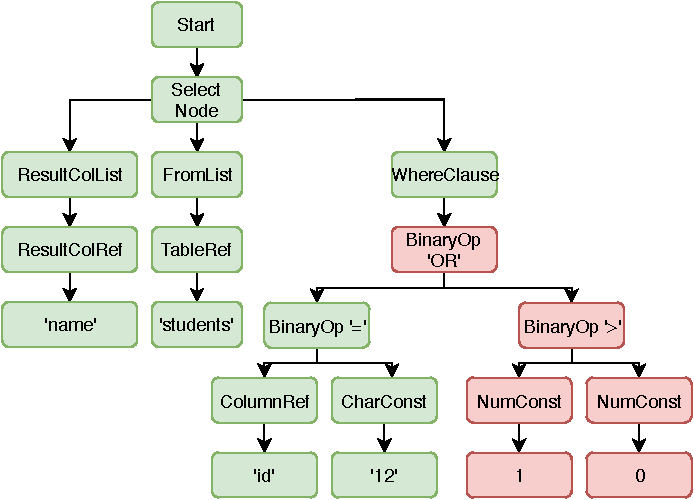
\includegraphics[width =0.8\linewidth]{images/sqlParseTreeInvalid.pdf}
\caption{SQL query parse tree} \label{invalidparsetree}
\end{figure}



\section{Summary}
This chapter first introduced a list of injection vulnerabilities considered in this work. Then, it presented a few static and dynamic approaches at detecting vulnerabilities.